\chapter{Problem Statement}\label{chap:problem}

\section*{}

This chapter describes the problem tackled in this dissertation, including the planned features and the expected result. First, it presents the features to be developed. Then, a set of proposed solutions are presented.

More information on how these features are planned to be executed is given on the next chapter.

\section{Problem Definition}\label{sec:prob-def}

As mentioned in the Introduction (Chapter~\ref{chap:intro}), the project's goal is to develop a web application that allows users to follow a sporting event in a real-time chat-like environment where everyone can input game events. For users that are just following, it would work as live coverage of the event; for contributors, it should be resilient to network failures due to stadiums' Wi-Fi limitations.
Due to the above goal, some necessary features start to surface, such as real-time conflict resolution and the inherent reputation system for tie-breaking when necessary. 

A prototype that allows event submission is already available, and since it is using React, which is an appropriate technology for this task, it will be kept. Some features still need to be polished, but most of the UI is already done, which will allow a bigger focus on the actual real-time conflict resolution problem.

The features of the prototype are described as follows, in User Story format\footnote{In software development and product management, a user story is an informal, natural language description of one or more features of a software system. User stories are often written from the perspective of an end-user or user of a system.}:

\begin{itemize}[leftmargin  = 3.25\parindent, align=left]
    \item[US01] As a user, I want to be able to join a sport event channel, where I can see details about the event in real-time (either pre-filled or contributed by other users), so that I have information about what is happening in the event.
    \item[US02] As a user, I want to be able to be able to post event updates while on an event channel, in a chat-like interaction, so that I can easily contribute in an input experience I recognize.
    \begin{itemize}
        \item Event updates include: Starting players, Goals, Fouls, Set-Pieces, Cards, Substitutions
    \end{itemize} 
    \item[US03] As a user, I want to be able to use the application while in offline mode, and have it synchronize once the connection is resumed, so that I don't lose information nor focus when my connection drops.
    \item[US04] As a user, I want to see a value representing the reputation of other users in a given event channel, so that I have a basis on which to decide if I trust them. 
    \item[US05] As a user, I want to be able to report input events as false, so that I can let others know that it might not be true and manifest my intention to change it.
    \item[US06] As a user, I want to be able to see if there are any pending conflicts to be resolved, so that I can clearly see if I need to solve any conflicting information.
    \item[US07] As a user, I want to be able to resolve any pending conflicts, so that I can keep the event's history clean and understandable.
    \item[US08] As a user, I want to be able to join an event channel mid-session, being able to see the previous information, so that I have more flexibility, not losing context if I arrive some time late.
\end{itemize}

\section{Problem Solution}\label{sec:prob-sol}

In this section, a preliminary approach for the problem is presented. In some cases, it is still not possible to make a clear decision, as it requires implementation and further testing to validate that it actually works and really fits the need. These proposed approaches are based on the research done in Chapter~\ref{chap:sota}, projected into the application domain and specific needs. This chapter is divided into sections, which will more precisely elaborate on their respective topic, presenting one or multiple proposed solutions for that specific area. 

\subsection{Knowledge Base}
This project will benefit from the existing structure of zerozero.pt knowledge base, and will integrate with it by pulling events data from it, as well as publishing the event inputs generated by the users, storing the event history.

\subsection{High Level Architecture}

Figure \ref{fig:high-level-arch} presents the proposed high level design for the application. The ZeroZero API is already available. The relevant parts are the ZeroZero Live Web Server, which will serve the web pages to the clients, mediating the state synchronization among them. It will communicate with the existing ZeroZero API for authentication and access to existing event information. It will also communicate with the other two micro-services. Reputation Service will handle the reputation calculation regarding the interactions during the event. Conflict Handling Service is responsible for handling the conflicts in real-time, resolving them automatically whenever possible, and cleaning up the event state. The Web clients will contain the frontend web pages with the logic to store changes locally and allow for offline working, as well as listening for the real-time updates to keep the state synchronized.

\begin{figure}[t]
    \begin{center}
        \leavevmode
        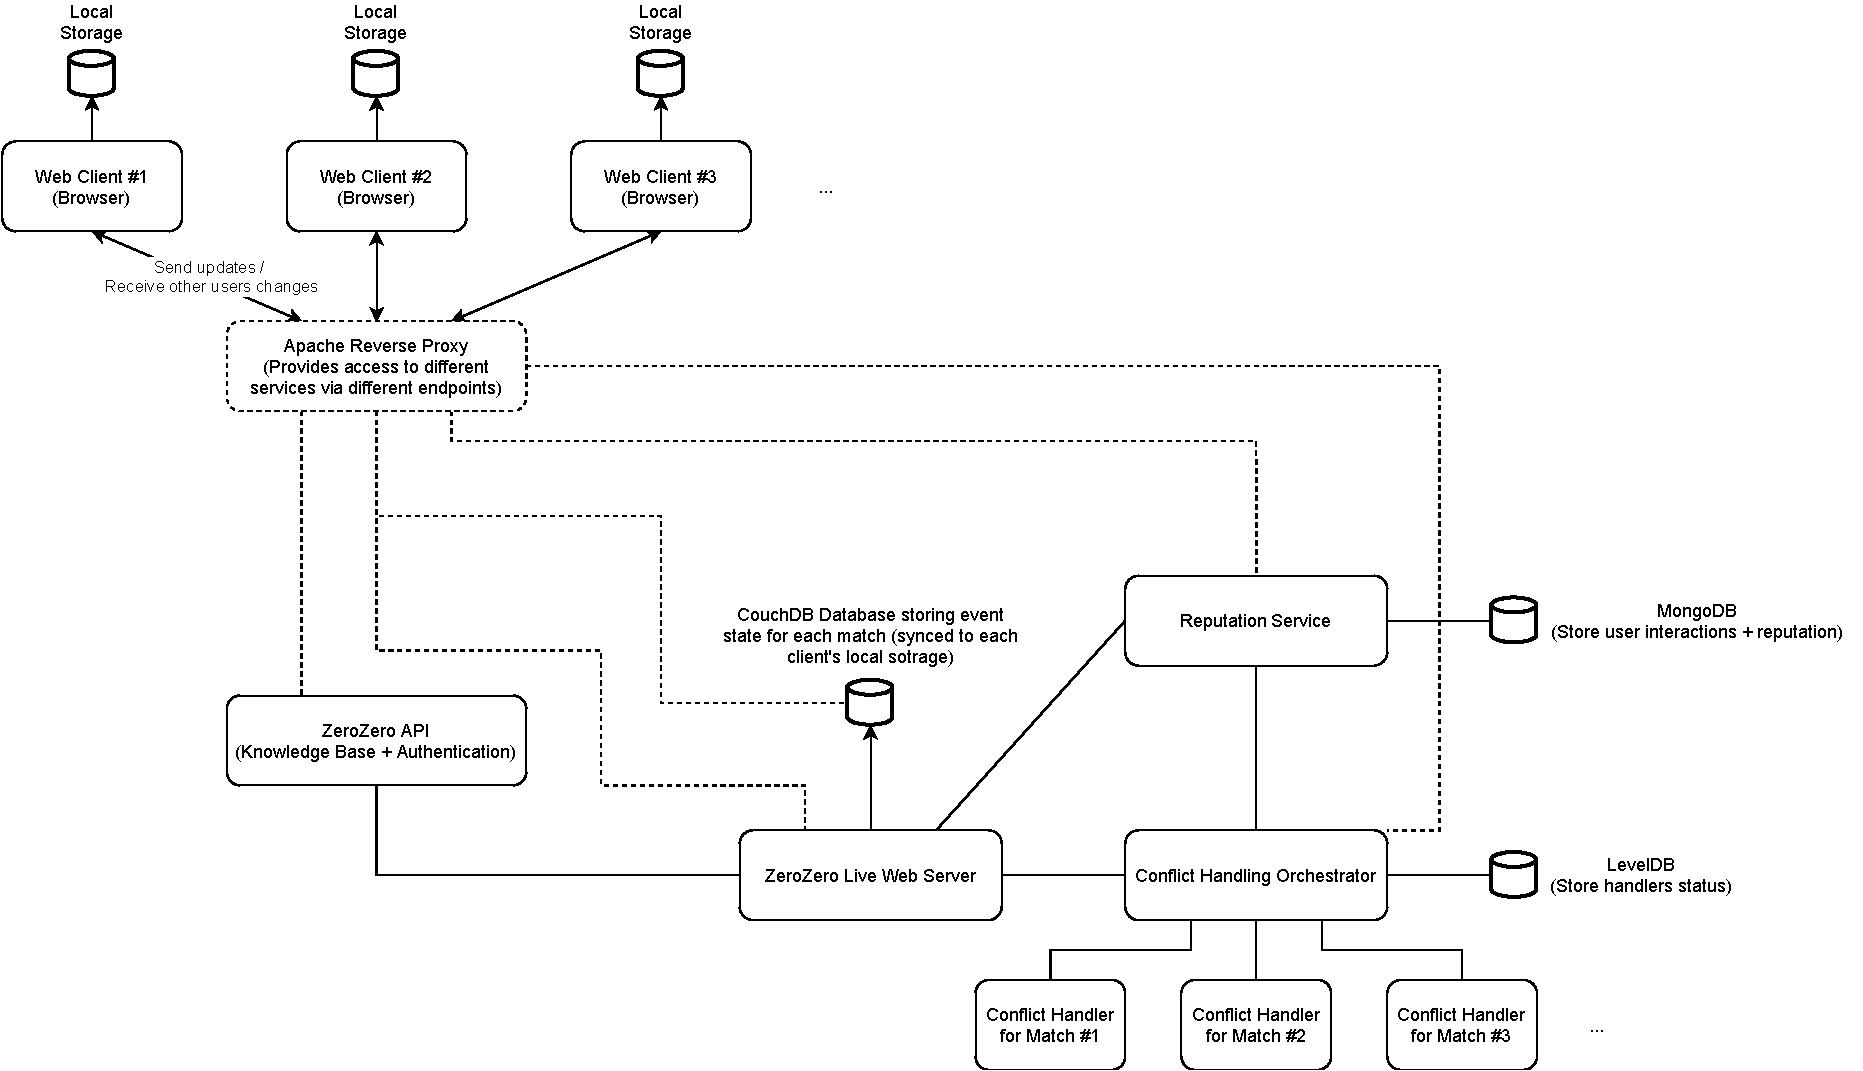
\includegraphics[width=0.9\textwidth]{zerozerolive-arch.pdf}
        \caption{High Level Architecture design of the zerozero.live system}
        \label{fig:high-level-arch}
    \end{center}
\end{figure}

\subsection{Offline Availability} \label{sec:prob-solution-offline-avail}
According to the research done in Chapter~\ref{chap:sota}, there needs to be a way of storing state locally if the user is offline. Since this application is a web application, from the alternatives presented, \textbf{localStorage} seems to be the most available among browsers\footnote{https://caniuse.com/?search=localstorage}, while fitting the project's needs. 

Currently, in the already existing \say{Proof-of-Concept}, there is an already implemented solution, which uses a local queue of requests stored in \textit{localStorage}, so as not to overwhelm the server with changes every second. This queue is \say{dumped} every 10 seconds. That is, every 10 seconds, the operations batched in the queue are sent to the server. While this allows for the prevention of operations loss in case of sudden network connectivity failure, it might not be the best approach in terms of real-time and user experience. For example, let's say that a user generates a conflicting operation, but that operation is only sent 10 seconds later. Only then will the user see that effect on their device, when it could have happened sooner.

My proposal is to reduce the waiting time to a more reasonable 2 seconds, which, while preventing the overwhelming of messages to the server, reduces notification time and still lets the user cancel the operation before it is sent.

\subsection{Conflict Resolution} \label{sec:prob-solution-conflict-res}
This is a topic on which there is no clear solution. As it was seen in the research, the most well-known and used approaches are OT and CRDT. The community cannot, however, elect a clear winner\footnote{https://news.ycombinator.com/item?id=22039950}, they are just \textit{different}. On the OT side, a common approach is to use ShareDB\footnote{https://github.com/share/sharedb}, together with the JSON OT type definition\footnote{https://github.com/ottypes/json0}.

Another alternative would be to use CouchDB\footnote{https://couchdb.apache.org/} with its web browser counterpart, PouchDB\footnote{https://pouchdb.com/}. It allows for replication of state among all users, with complete control on conflict resolution: When CouchDB encounters a conflict scenario, it arbitrarily chooses a winner, deterministically; however, it keeps the conflicting version as well, which can be used to solve the conflict with custom application logic, for example, based on a reputation system, or on merging the two inputs --- Creative Resolution (Section~\ref{sec:conflict-res-sota})

On the CRDT side, there are two options: Automerge\footnote{https://github.com/automerge/automerge} and GUN\footnote{https://github.com/amark/gun}. Since the latter's documentation seems to be lacking, I am removing it from the options pool. Automerge is flexible enough, allowing for server-client network architecture, as well as peer-to-peer, and it works like JSON CRDT were described to work: each user has a local copy of the JSON state, which can be locally mutated, even when offline, and it will sync automatically with other nodes. It works similarly to the CouchDB/PouchDB conflict handling, in being as much automatic as possible but letting the application know about existing conflicts and handle them.

At this point, the ShareDB option seems to work on a lower level than the other two, and it might be unfeasible to have good results in the expected timeframe. Between CouchDB/PouchDB and Automerge, there is no clear winner, the only distinctive characteristic being that CouchDB is more mature and has been used in production for much longer. Nevertheless, the wise decision here would be to try both in a small \say{Proof-of-Concept} and further verify their usability. 

\subsection{Reputation System} \label{sec:problem-solution-rep-sys}
As was mentioned in the Literature Review (Section~\ref{sec:rep-sys-sota}), an effective method to achieve a fair reputation system, which takes into account the time dynamics of user interactions as well as their current reputation, is to implement a personalized PageRank algorithm. It takes into account the reputation of users when calculating vouching or invalidation in order to achieve a weighted voting system so as to provide long-term reputable users with a prize for their good behavior. Recalling the system present in \cite{Daly2009}, there are 4 rules involved in adapting the system to our use case:

\begin{enumerate}
    \item Every time a user consumes a document from an author, the author gains reputation;
    \item Every time a user consumes a document, the document gains \say{reputation} (i.e.,\ popularity);
    \item In order to take time dynamics into account, reputation should decrease over time, so that a \say{rich-get-richer} paradigm can be avoided (both for users and for documents);
    \item Users with higher reputation matter more when calculating the document reputation changes;
\end{enumerate}

With this in mind, I propose the following rules to adapt this to our scenario:

\begin{itemize}
    \item Every time a user agrees with an input, he will improve the input's reputation according to rules 2 and 4;
    \begin{multline} \label{eq:rep-inc-proposal}
        newIR = oldIR + (1 - oldIR) * maxRepReward * userRep * userRepInfluence
    \end{multline}
    where $IR$ means \textit{Input Reputation}
    \item Every time a user disagrees with an input (either by inputting a real-conflicting input or reporting as false/inaccurate) he will worsen the input's rep according to rules (2's reverse) and 4;
    \begin{equation}
        newIR = oldIR * (1 - maxRepPunishment * userRep * userRepInfluence)
    \end{equation}
    \item Every time a user submits a falsely-conflicting input, meaning that both users submitted the same information resulting in duplicated information, it should act as an explicit agreement with the other user's input, so it should count more, according to an $explicitAgreementBonus$ constant, which must be greater than zero to achieve the bonus effect;
    \begin{equation}
    newIR = baseIRIncrement * (1 + explicitAgreementBonus)
    \end{equation}
    where $baseIRIncrement$ is calculated based on \ref{eq:rep-inc-proposal}
    \item The user gains reputation according to the average of its inputs' reputations. Only takes into account the latest inputs, referring to the last event which will trigger the reputation update;
    \begin{equation}
        newUserRep = oldUserRep + (1 - oldUserRep) * \frac{\sum IR}{numInputs}
    \end{equation}
    \item Each user has a reputation decay according to rule no. 3, the time unit should be 1 week since there's at least one relevant game per week. This prevents users that generate a lot of inputs in a single game to enjoy their reputation boost for many more games, since they need to be consistent every week: it matters more if they make an input every week than 20 inputs once every 2 or more weeks.
    This decay is on a higher level than the events, creating 20 inputs in an event is roughly the same as 1 input in an event (since the football events last around 90 minutes)
    \begin{equation}
        newUserRep = oldUserRep * decayCoefficient^{timeSinceLastUpdate}
    \end{equation}
    \item The reputation values are updated at the end of each event, according to the event's history.
\end{itemize}

\subsection{Automated Testing}

When testing a usual single-user Web Application, we rely on the simulation of user actions such as clicking on components, inputting information and submitting forms. Then we assert what we expect those actions to change on the webpage. This can be done as unit tests, where we simulate the rendering of the webpage, generating the DOM, then simulate the actions and their effects on the DOM, and finally assert on how the DOM should look like in the end. 

A more complex scenario is simulating the whole browser, which can interact with actual web servers, as if actual users were requesting the page, commonly known as end-to-end testing.

However, since we aim to test a multi-user application, we should consider that in the test scenarios themselves, having multiple agents execute specific actions on specific times, to trigger conflict situtations.

In order to do this, all agents must be connected to the same event, and thus need to connect to a server, which will host a test event. Additionally, all agents must be able to execute concurrent actions on demand. For this, I propose the implemtation of an orchestrator entity which controls the agents running the browser engine simulation. The test cases would include a relative timestamp, so that actions with the same timestamp should be executed concurrently.

Finally, the agents would assert on their application view, and report to the orchestrator, which would join the results and coordinate the test suite.

More specifically, this allows us to request two agents to submit two conflicting inputs and assert that both of them see the conflict and are able to solve it.

\section{Summary}

In summary, the problem to be tackled is the development of a multi-user real-time application allowing the coverage of sporting events, with offline tolerance. That entails the existance of conflict resolution strategies, as well as a reputation system, which should take time into consideration, making reputation more dynamic.

The automated testing of such an application is not trivial, since it will require the simulation of multiple agents executing the actions the real users would do. They must be managed by an orquestrator service that will synchronize their actions, based on the event time, which can then simulate concurrent events.


